%% ============================================================
%%  EpiSentinel — IEEE Two-Column Conference Paper
%%  Authors: Ekansh Nandan Sharma, GN Disha, Ishan Mahajan,
%%           Prof. Saraswathi Govind Datar
%%  Institution: RV College of Engineering, Bengaluru, India
%% ============================================================
\documentclass[conference]{IEEEtran}
\IEEEoverridecommandlockouts

%% ---- Package imports ----------------------------------------
\usepackage{cite}
\usepackage{amsmath,amssymb,amsfonts}
\usepackage{algorithmic}
\usepackage{graphicx}
\usepackage{textcomp}
\usepackage{xcolor}
\usepackage{booktabs}
\usepackage{array}
\usepackage{multirow}
\usepackage{url}
\usepackage{hyperref}
\usepackage{microtype}
\usepackage{balance}
\usepackage[T1]{fontenc}
\usepackage{lmodern}

%% ---- TikZ for system diagram --------------------------------
\usepackage{tikz}
\usetikzlibrary{shapes.geometric, arrows.meta, positioning,
                fit, backgrounds, calc, shadows}

%% ---- Hyperref config (suppress colour boxes in print) -------
\hypersetup{
  colorlinks = true,
  linkcolor  = blue!60!black,
  citecolor  = blue!60!black,
  urlcolor   = blue!60!black
}

%% ---- Column-width helper ------------------------------------
\newcolumntype{C}[1]{>{\centering\arraybackslash}p{#1}}
\newcolumntype{L}[1]{>{\raggedright\arraybackslash}p{#1}}

%% =============================================================
\begin{document}

\title{\textbf{EpiSentinel:} An Explainable Ensemble Framework with
Autoregressive Epidemiological Signals and SOP-Grounded Advisory for
District-Level Dengue Outbreak Forecasting in Karnataka, India}

\author{%
  \IEEEauthorblockN{Ekansh Nandan Sharma}
  \IEEEauthorblockA{%
    \textit{Department of Computer Science Engineering}\\
    RV College of Engineering, Bengaluru, India\\
    \texttt{ekanshnandans.cs25@rvce.edu.in}}
  \and
  \IEEEauthorblockN{GN Disha}
  \IEEEauthorblockA{%
    \textit{Department of Computer Science Engineering}\\
    RV College of Engineering, Bengaluru, India\\
    \texttt{gndisha.cs25@rvce.edu.in}}
  \and
  \IEEEauthorblockN{Ishan Mahajan}
  \IEEEauthorblockA{%
    \textit{Department of Computer Science Engineering}\\
    RV College of Engineering, Bengaluru, India\\
    \texttt{ishanmahajan.cs25@rvce.edu.in}}
  \and
  \IEEEauthorblockN{Prof.\ Saraswathi Govind Datar}
  \IEEEauthorblockA{%
    \textit{Department of Computer Science Engineering}\\
    RV College of Engineering, Bengaluru, India\\
    \texttt{saraswathigd@rvce.edu.in}}
}

\maketitle

%% ============================================================
\begin{abstract}
Dengue fever imposes a substantial and growing burden on public
health systems across tropical and subtropical regions. In Karnataka,
India, conventional surveillance infrastructure---anchored by the
Integrated Disease Surveillance Programme (IDSP) and the National
Vector Borne Disease Control Programme (NVBDCP)---operates in a
reactive mode: outbreak reports typically arrive two to three weeks
after transmission peaks, leaving health systems unable to pre-position
resources. We present \textbf{EpiSentinel}, a district-level binary
outbreak classification system that delivers seven-day advance
forecasts across approximately 30 Karnataka districts.

The core methodological novelty lies in an explicitly
\emph{autoregressive} feature design: lagged case series and
rolling epidemiological averages serve as the \emph{primary}
predictors, with climate features acting as modulating covariates.
SHAP attribution confirms that the three top-ranked features are all
autoregressive epidemiological signals, contributing collectively
2.8$\times$ more predictive weight than the highest-ranked climate
variable. A weighted ensemble of XGBoost, CatBoost, LightGBM, Random
Forest, and a Poisson regressor is calibrated with locally-defined
per-district outbreak thresholds derived from each district's own
historical case distribution, avoiding the aggregation bias that
afflicts uniform national thresholds.

We introduce a systematic three-stage leakage audit methodology
for district-level panel data---identifying and removing direct
geographic identifiers, demographic proxies, and historical
statistical proxies---and demonstrate that its omission inflates
apparent ROC-AUC by approximately 3--4 percentage points.
Calibrated 90\% conformal prediction intervals (implemented via
MapieClassifier) accompany each risk score, providing health officers
with principled uncertainty bounds. An explainable dashboard surfaces
per-prediction SHAP feature drivers, and a Retrieval-Augmented
Generation (RAG) advisory layer converts risk scores into
SOP-grounded action plans via Gemini-1.5-Flash and LangChain,
with domain-scoped guardrails preventing hallucinated responses.

On a held-out 2023 test set (hard temporal split), the final ensemble
achieves \textbf{ROC-AUC 0.821}, \textbf{PR-AUC 0.825},
\textbf{Recall 0.856}, and \textbf{F1 0.720}, with a threshold chosen
to enforce Recall $\geq 0.85$ reflecting the asymmetric cost of missed
outbreaks in public health deployments.
\end{abstract}

\begin{IEEEkeywords}
dengue forecasting, conformal prediction, SHAP explainability,
autoregressive epidemiological signals, ensemble learning,
retrieval-augmented generation, Karnataka surveillance, leakage audit,
uncertainty quantification, public health decision support
\end{IEEEkeywords}

%% ============================================================
\section{Introduction}
\label{sec:intro}

Dengue fever is the world's fastest-spreading vector-borne disease.
The World Health Organization estimates that 3.9~billion people in
more than 130 countries are at risk, with approximately 390~million
infections occurring annually, of which 96~million manifest clinical
illness \cite{who_dengue}. India accounts for an outsized share of
this burden: the NVBDCP reported over 228,000 dengue cases and 303
deaths during 2022 alone \cite{nvbdcp2022}, though passive
surveillance is widely believed to undercount true incidence by a
factor of 10--30$\times$ \cite{kakarla2023}.

Karnataka, located in southern India, experiences pronounced seasonal
dengue transmission driven by the Southwest Monsoon (June--September)
and a secondary post-monsoon surge (October--November).
The state's 31 administrative districts present highly heterogeneous
transmission environments---from the dense urban core of Bengaluru
Urban (population $>$11.4~million) to the sparsely populated
hill districts of Kodagu and Chikkamagaluru---meaning that a case
count that constitutes a minor background signal in one district
may represent a serious outbreak in another.

\subsection{The Reactive Surveillance Gap}

Under the current IDSP/NVBDCP reporting structure, district-level
case counts are compiled from health facility records, aggregated at
the district level, and transmitted to state and national dashboards.
This pipeline introduces a structural lag: reports typically reach
decision-makers two to three weeks \emph{after} an outbreak has
already peaked \cite{nvbdcp2022}. By the time a health authority
identifies a surge and deploys vector-control personnel, larvicide
stock, and clinical capacity, the transmission peak may have already
passed---and the window for meaningful early intervention is lost.

\subsection{The Biological Case for 7-Day Forecastability}

The transmission biology of \textit{Aedes aegypti}-mediated dengue
creates a compressible window of predictability that our system
exploits. The causal chain proceeds as follows:

\begin{enumerate}
  \item A rainfall or humidity spike creates standing water, the
        primary breeding habitat for \textit{Ae.\ aegypti} (0--2 days).
  \item Larvae develop to adult mosquitoes under warm, humid
        conditions (7--10 days).
  \item A newly hatched mosquito bites a viraemic host and undergoes
        extrinsic incubation of the dengue virus (8--14 days, temperature
        dependent).
  \item An infected mosquito transmits virus to a susceptible human,
        who develops clinical dengue after an intrinsic incubation of
        4--7 days.
\end{enumerate}

The full chain from environmental trigger to clinical presentation
spans approximately 19--33 days. Critically, however, once active
community transmission is underway---already reflected in
\emph{current} case counts---the ``momentum'' encoded in the
existing infection pool directly predicts near-term case counts
with a shorter, more reliable lead time. It is this momentum,
captured by lagged case series and rolling averages, that our
autoregressive design deliberately foregrounds.

\subsection{Limitations of Existing ML Approaches}

The majority of published ML-based dengue forecasting systems model
case counts as a function of climate variables alone: temperature,
humidity, rainfall, and their lags \cite{kakarla2023, sebastianelli2024,
iitm2025}. While climate is an important \emph{structural} driver of
epidemic suitability, it fails to capture \emph{active} transmission
dynamics. When dengue is actively spreading in a district, lagged
case counts encode this dynamic far more directly than temperature
forecasts. Our SHAP analysis (Section~\ref{sec:shap}) empirically
confirms this: autoregressive features outrank all climate features
by a factor of 2.8$\times$ at a 7-day horizon.

A second limitation of existing systems is the absence of systematic
leakage auditing for panel-structured epidemiological data. Features
such as fixed district identifiers, 2011 census population counts
(constant per district across the panel), or district-level case
statistics computed from the full dataset can silently encode
geographic identity, causing models to memorise per-district
base rates rather than learning transferable transmission dynamics.
We formalise a three-stage leakage audit methodology
(Section~\ref{sec:leakage}) and demonstrate its impact quantitatively.

\subsection{Contributions}

This paper makes the following contributions:

\begin{enumerate}
  \item \textbf{Autoregressive design}: We demonstrate, backed by
        global SHAP analysis, that lagged case series and rolling
        epidemiological averages are the dominant 7-day-ahead signals,
        establishing a principled design prior for short-horizon
        outbreak forecasting.

  \item \textbf{Three-stage leakage audit}: A systematic methodology
        for identifying and removing direct geographic identifiers,
        demographic proxies, and historical statistical proxies from
        district-level panel data---proposed as a reusable standard
        for epidemiological ML pipelines.

  \item \textbf{Per-district threshold calibration}: Binary outbreak
        labels defined relative to each district's own case
        distribution, correcting for heterogeneous baseline
        transmission intensity.

  \item \textbf{Conformal uncertainty quantification}: District-level
        90\% prediction intervals via split-conformal calibration,
        surfaced in the dashboard alongside point risk scores.

  \item \textbf{SOP-grounded RAG advisory}: A domain-scoped LLM
        layer that translates risk scores into actionable,
        protocol-anchored response recommendations---the first
        published system to pair ML outbreak prediction with a
        guardrailed SOP advisory interface.

  \item \textbf{Open-source end-to-end implementation}: The full
        pipeline---training, evaluation, SHAP, conformal wrapper,
        FastAPI backend, and D3.js dashboard---is publicly available.
\end{enumerate}

%% ============================================================
\section{Related Work}
\label{sec:related}

\subsection{Climate-Driven Dengue Forecasting}

Early computational dengue forecasting relied on mechanistic
compartmental models (SIR/SEIR) driven by temperature and rainfall
inputs. Machine learning approaches superseded these for predictive
accuracy. Kakarla \textit{et al.} \cite{kakarla2023} trained Random
Forest and gradient boosting models across Indian states using
lagged rainfall and temperature indices, achieving reasonable district-
level correlation but noting that model performance degraded in years
with anomalous monsoon timing. Sebastianelli \textit{et al.}
\cite{sebastianelli2024} demonstrated a reproducible ensemble pipeline
using Sentinel-2 satellite imagery and meteorological reanalysis,
showing that vegetation and water-body indices add predictive value
for \textit{Aedes} habitat suitability. The IITM Pune group
\cite{iitm2025} employed LSTM networks to produce two-month dengue
forecasts at the state level for India, leveraging ERA5 climate
reanalysis and demonstrating strong seasonal skill.

A common limitation across these works is their treatment of climate
as the \emph{primary} and often \emph{exclusive} predictive signal.
While climate sets the boundary conditions for epidemic suitability,
it cannot encode whether active community transmission is occurring
at the time of forecasting. At a 7-day prediction horizon---the
operationally relevant window for resource pre-positioning---the
current infection pool is a far stronger predictor. Our system
addresses this gap by explicitly prioritising autoregressive
epidemiological features.

\subsection{Ensemble Machine Learning for Outbreak Prediction}

The superiority of heterogeneous ensembles over single-model
approaches for tabular epidemiological data has been established
across several disease contexts. A recent ScienceDirect study
applied XGBoost and LightGBM ensembles to dengue prediction in
Bangladesh, incorporating SHAP and LIME explainability to improve
clinician trust \cite{bangladesh_xai2025}. Their results demonstrate
the practical benefit of combining gradient boosting with a
post-hoc explainability layer. Our system extends this line of work
by (a) optimising ensemble weights via Dirichlet sampling on a
held-out validation year rather than simple averaging, (b) including
a Poisson regressor alongside classifiers to capture count-process
dynamics, and (c) calibrating decision thresholds per district rather
than globally.

\subsection{Explainability in Epidemiological Machine Learning}

Shapley Additive Explanations (SHAP), introduced by Lundberg and Lee
\cite{lundberg2017}, provide a theoretically grounded framework for
attributing model predictions to individual features based on
cooperative game theory. TreeSHAP \cite{lundberg2020} extends this to
tree ensemble models with polynomial-time exact computation, making
it practical for the multi-model ensemble setting. SHAP has been
applied to tuberculosis risk prediction \cite{iitm2025}, COVID-19
severity scoring, and dengue hotspot identification
\cite{bangladesh_xai2025}. A key finding across these applications is
that SHAP values serve not only as a diagnostic tool for model
developers but as a communication medium for health officers---enabling
the translation of opaque model outputs into actionable, feature-
level explanations. EpiSentinel surfaces per-prediction top-driver
SHAP values in the dashboard alongside each district's risk score.

\subsection{Large Language Models and RAG in Public Health}

The integration of Large Language Models (LLMs) into epidemiological
intelligence is an active frontier. The PandemicLLM framework
\cite{frontiersai2025} demonstrated that LLMs fine-tuned on
epidemiological literature can generate plausible outbreak
narratives, though hallucination risk remains a central concern
for safety-critical deployments. Retrieval-Augmented Generation (RAG)
\cite{rag_healthcare2025} addresses this by grounding LLM responses
in retrieved document context, substantially reducing factual errors
for domain-specific queries. Despite this progress, no published
system to our knowledge combines a validated ML outbreak prediction
model with an SOP-grounded RAG advisory layer featuring domain-
scoped guardrails---the gap EpiSentinel's Sentinel AI component
directly addresses.

%% ============================================================
\section{Dataset and Feature Engineering}
\label{sec:data}

\subsection{Dataset Description}

The EpiSentinel training corpus is a balanced panel dataset
structured as $(d, t)$ tuples, where $d$ denotes an administrative
district and $t$ an ISO epidemiological week. The dataset spans
Karnataka's approximately 30 districts from 2017 through 2023, yielding
a base population of approximately $30 \times 52 \times 7 \approx 10{,}920$
district-week observations. After application of quality filters
described below, the usable panel is approximately 9,153 rows.

Dengue case and death data were sourced from IDSP and NVBDCP
surveillance records, aggregated at weekly district resolution.
Meteorological covariates (temperature, humidity, rainfall) were
obtained from India Meteorological Department gridded products
and spatially averaged to district centroids. Population data were
drawn from WorldPop 2020 gridded population surfaces
\cite{worldpop}, providing time-varying population estimates at
100\,m resolution.

The temporal split follows a strict calendar boundary:
\textbf{Training: 2017--2021}, \textbf{Validation: 2022},
\textbf{Test: 2023}. No data from 2022 or 2023 participates in
model training or hyperparameter selection, ensuring the test
set constitutes a genuine out-of-sample evaluation.

Two data quality flags were applied. First, \texttt{is\_unreliable
\_2017\_peak\_week} identifies weeks during the anomalously large
2017 outbreak in Karnataka, during which reporting mechanisms were
known to be under exceptional strain; these rows are excluded from
training to prevent the model from learning an unrepresentative
transmission regime. Second, \texttt{exclude\_training\_row} captures
additional rows identified during EDA as structurally unreliable
(e.g., weeks with imputed zero counts due to missing reports). Both
flags are applied during training and cross-validation but are not
required at inference time.

\subsection{Target Variable Definition}
\label{subsec:target}

The binary outbreak label is defined per district using a
locally-calibrated threshold. Let $C_{d,t}$ denote the reported
dengue case count for district $d$ in ISO week $t$, and let
$\mathcal{T}_{\text{train}}$ denote the set of all training weeks.
Define the per-district 75th percentile over training weeks as:

\begin{equation}
  Q_{75}^{d} = \text{quantile}_{0.75}
  \left\{ C_{d,t} \;\middle|\; t \in \mathcal{T}_{\text{train}} \right\}
  \label{eq:q75}
\end{equation}

The binary target for the \emph{following} week's outbreak status is
then:

\begin{equation}
  y_{d,t} = \begin{cases}
    1 & \text{if } C_{d,t+1} > Q_{75}^{d} \\
    0 & \text{otherwise}
  \end{cases}
  \label{eq:target}
\end{equation}

This formulation has two critical properties. First, \emph{local
calibration}: rather than applying a uniform national threshold,
each district's outbreak label is defined relative to its own
historical distribution. A count of 15 cases may represent a
routine week for Bengaluru Urban but a severe outbreak event for
Kodagu, whose 75th percentile is substantially lower; uniform
thresholds would systematically mislabel such districts. Second,
\emph{temporal integrity}: $Q_{75}^{d}$ is computed exclusively
from training-set weeks. It is never used as a model feature
(see Section~\ref{sec:leakage} for the formal leakage audit),
ensuring that future case distribution information cannot leak
into the model's input space.

\subsection{Feature Groups}
\label{subsec:features}

Table~\ref{tab:features} presents the complete set of features
grouped by category, with biological and epidemiological rationale
for each group.

\begin{table}[htbp]
  \caption{Feature Groups with Epidemiological Rationale}
  \label{tab:features}
  \centering
  \renewcommand{\arraystretch}{1.15}
  \setlength{\tabcolsep}{4pt}
  \begin{tabular}{L{1.6cm} L{3.0cm} L{2.8cm}}
    \toprule
    \textbf{Group} & \textbf{Features} & \textbf{Rationale} \\
    \midrule
    Epidem.\ current &
      \texttt{dengue\_cases\_reported},
      \texttt{deaths\_weekly},
      \texttt{cases\_per\_100k} &
      Current case burden; incidence rate normalises for district size \\
    \midrule
    Autoregressive lags &
      \texttt{cases\_lag1},
      \texttt{cases\_lag2},
      \texttt{cases\_lag3} &
      Captures active transmission momentum; within the intrinsic
      incubation window ($\sim$7 days) \\
    \midrule
    Rolling averages &
      \texttt{cases\_roll2\_mean},
      \texttt{cases\_roll4\_mean} &
      Smooths reporting noise; 4-week average captures sustained outbreak
      trajectory \\
    \midrule
    Current climate &
      \texttt{temp\_mean\_week},
      \texttt{humidity\_mean\_week},
      \texttt{rainfall\_total\_week},
      \texttt{temp\_max\_week},
      \texttt{humidity\_max\_week} &
      Weekly climate conditions affecting mosquito survival and
      activity \\
    \midrule
    Lagged climate &
      \texttt{temp\_mean\_lag1/2},
      \texttt{humidity\_mean\_lag1/2},
      \texttt{rainfall\_total\_lag1/2} &
      Extrinsic incubation period $\approx$10--14 days means climate
      2 weeks prior is most informative \\
    \midrule
    Seasonality &
      \texttt{week\_sin},
      \texttt{week\_cos} &
      Circular encoding preserves continuity at year boundary;
      captures monsoon and post-monsoon dengue peaks \\
    \midrule
    Population &
      \texttt{worldpop\_total},
      \texttt{worldpop\_density\_per\_km2} &
      Time-varying population scale and density; density determines
      transmission rate via human contact frequency \\
    \bottomrule
  \end{tabular}
\end{table}

\subsection{Seasonality Encoding}
\label{subsec:seasonality}

Raw ISO week number $w \in \{1, \ldots, 52\}$ is a poor predictor
because it treats weeks 52 and 1 as numerically distant despite
their temporal adjacency. To preserve the circular structure of the
annual cycle, we apply the encoding:

\begin{equation}
  \texttt{week\_sin} = \sin\!\left(\frac{2\pi w}{52}\right),
  \quad
  \texttt{week\_cos} = \cos\!\left(\frac{2\pi w}{52}\right)
  \label{eq:seasonality}
\end{equation}

The pair $(\texttt{week\_sin},\; \texttt{week\_cos})$ forms a
unit-circle coordinate that maps any two epidemiologically
adjacent weeks to nearby points in $\mathbb{R}^2$, regardless of
whether they straddle the year boundary. This encoding is
particularly important for Karnataka, where the post-monsoon dengue
surge (weeks 42--48) immediately precedes a low-transmission period
that begins around week 52 and continues into the early weeks of the
following calendar year.

%% ============================================================
\section{Systematic Identification and Removal of Geographic
         Identity Proxies}
\label{sec:leakage}

Leakage auditing is a standard practice in supervised learning, but
its application to \emph{district-level panel data} requires special
attention because geographic identity can be silently re-encoded
through features that appear superficially benign. We formalise a
three-stage audit and demonstrate quantitatively that omitting it
inflates reported model performance.

\subsection{Stage 1 --- Direct Geographic Identifier}

\textbf{Feature:} \texttt{district} (categorical string label).

\textbf{Leakage mechanism:} A tree-based model trained on this
feature can partition the tree on district identity and effectively
memorise per-district historical outbreak base rates from the
training data. This creates a shortcut that bypasses the epidemiological
signal structure entirely: the model simply learns ``District $d$ has
historically been high-risk'' rather than ``a given combination of
current features implies high risk in district $d$.'' Such a model
will fail silently when deployed in a district with a shifting
epidemiological profile or extended to a new district.

\textbf{Detection:} Drop-one ablation experiments showed a
disproportionately large performance decline (approximately 4--5
percentage points in F1) when the \texttt{district} feature was
removed versus dropping any other single feature, confirming its
dominant role as a district-identity shortcut.

\textbf{Resolution:} \texttt{district} is removed entirely from all
model training, hyperparameter search, and inference pipelines.

\subsection{Stage 2 --- Demographic Proxy}

\textbf{Feature:} \texttt{population\_2011} (2011 census total
population, a constant value per district).

\textbf{Leakage mechanism:} A feature that is strictly constant
within the time series of a single district carries zero within-
district temporal information. It is therefore equivalent, from the
model's perspective, to a numeric district identifier. Each of
Karnataka's districts has a unique 2011 census population; when this
feature is included, the model can recover district identity from a
single numeric column and replicate the memorisation shortcut
described in Stage 1.

\textbf{Detection:} SHAP global importance analysis placed
\texttt{population\_2011} among the top-ranked features despite its
theoretical inability to convey within-district temporal variation.
This anomalous ranking is the diagnostic signature of a proxy
leakage feature.

\textbf{Resolution:} \texttt{population\_2011} is removed.
The time-varying WorldPop 2020 estimate (\texttt{worldpop\_total})
is retained, as it varies year-to-year and does not have a unique
mapping to district identity.

\subsection{Stage 3 --- Historical Statistical Proxy}
\label{subsec:q75_leakage}

\textbf{Feature:} \texttt{district\_case\_q75} (the per-district
75th percentile case count, computed from the full dataset history).

\textbf{Leakage mechanism:} This is the most subtle and insidious
form of leakage. Although the feature appears to describe a
statistical property of the case distribution rather than identity
per se, it possesses a \emph{unique value for each district in the
panel}. The mapping $d \mapsto Q_{75}^{d}$ is therefore a
deterministic bijection from district identity to a float. Including
this feature is mathematically equivalent to including the district
string label---the model receives district identity as a floating-
point number. Furthermore, the feature is computed from the full
2017--2023 dataset, meaning it incorporates information from the
2022 and 2023 validation and test periods. This constitutes
\emph{future leakage} in addition to identity leakage.

\textbf{Detection:} When \texttt{district\_case\_q75} was included,
the ensemble ROC-AUC on the 2023 test set was approximately 0.85+.
Removing it reduced ROC-AUC to the honest value of 0.821---a
decrease of approximately 3--4 points that reflects the elimination
of the shortcut.

\textbf{Resolution:} \texttt{district\_case\_q75} is used
exclusively for \emph{label generation} (Equation~\ref{eq:q75})
and is never included as a model input feature at any stage.

\subsection{Additional Exclusions}

Two further features are excluded for related reasons:

\begin{itemize}
  \item \texttt{year}: Temporal leakage. Including calendar year
    as a feature allows the model to learn year-specific reporting
    artefacts or epidemic patterns with no generalisable meaning
    at deployment time.
  \item \texttt{is\_unreliable\_2017\_peak\_week}: An audit flag
    generated during data cleaning that is not available at
    inference time.
\end{itemize}

\subsection{Quantitative Impact of the Leakage Audit}

Table~\ref{tab:leakage} shows the measured performance impact of
each feature class on the 2023 held-out test set.

\begin{table}[htbp]
  \caption{Performance Inflation from Leaky Features (2023 Test Set)}
  \label{tab:leakage}
  \centering
  \renewcommand{\arraystretch}{1.15}
  \setlength{\tabcolsep}{5pt}
  \begin{tabular}{lcccc}
    \toprule
    \textbf{Feature Configuration} &
    \textbf{ROC-AUC} & \textbf{Recall} & \textbf{F1} \\
    \midrule
    With \texttt{district} (label)         & 0.864 & 0.891 & 0.779 \\
    + \texttt{population\_2011}            & 0.858 & 0.883 & 0.764 \\
    + \texttt{district\_case\_q75}         & 0.852 & 0.880 & 0.759 \\
    \textbf{Audit-clean (ours)}            & \textbf{0.821} &
                                             \textbf{0.856} &
                                             \textbf{0.720} \\
    \bottomrule
  \end{tabular}
\end{table}

The three-stage audit we propose---\emph{direct identifiers,
demographic proxies, historical statistical proxies}---constitutes
a reusable methodology for any district-level epidemiological ML
pipeline. Geographic identity leakage is particularly insidious in
panel data structures because the shortcut features are distributed
across multiple apparently distinct feature types.

%% ============================================================
\section{Model Development and Experiments}
\label{sec:models}

\subsection{Experimental Progression}

Model development proceeded through four experimental configurations,
each building on lessons from the preceding iteration.

\textbf{Run A --- Baseline Individual Models (with Population Features).}
Five models were independently trained and evaluated on 2023 test
data with a common feature set including \texttt{worldpop\_total}
and \texttt{worldpop\_density\_per\_km2} but no district label or
census proxies. Table~\ref{tab:run_a} presents results. CatBoost
and Random Forest achieve the highest individual ROC-AUC values at
this stage (0.826 and 0.818 respectively). The Poisson regressor,
adapted for binary prediction by normalising its count output,
substantially underperforms (ROC-AUC 0.481), confirming that a
pure count model is poorly matched to the binary outbreak
classification objective.

\begin{table}[htbp]
  \caption{Run A --- Individual Model Performance (2023 Test Set)}
  \label{tab:run_a}
  \centering
  \renewcommand{\arraystretch}{1.15}
  \setlength{\tabcolsep}{3pt}
  \begin{tabular}{lcccccc}
    \toprule
    \textbf{Model} & \textbf{Thresh.} & \textbf{ROC} &
    \textbf{PR} & \textbf{Prec.} & \textbf{Rec.} & \textbf{F1} \\
    \midrule
    CatBoost       & 0.25 & 0.826 & 0.829 & 0.687 & 0.769 & 0.725 \\
    XGBoost        & 0.16 & 0.817 & 0.820 & 0.630 & 0.820 & 0.712 \\
    LightGBM       & 0.16 & 0.809 & 0.814 & 0.658 & 0.772 & 0.710 \\
    Random Forest  & 0.22 & 0.818 & 0.825 & 0.609 & 0.846 & 0.708 \\
    Poisson Regr.  & ---  & 0.481 & 0.455 & 0.669 & 0.692 & 0.680 \\
    \bottomrule
  \end{tabular}
\end{table}

\textbf{Run B --- Weighted Ensemble after Leakage Fix.}
After removing \texttt{district}, \texttt{population\_2011}, and
\texttt{district\_case\_q75} as described in Section~\ref{sec:leakage},
a weighted ensemble was constructed (see Section~\ref{subsec:ensemble}).
Table~\ref{tab:run_b} shows that the ensemble outperforms all
individual models on F1 (0.720), demonstrating the complementarity
of the constituent learners even after leakage correction.

\begin{table}[htbp]
  \caption{Run B --- Weighted Ensemble and Individual Models
           after Leakage Fix (2023 Test Set)}
  \label{tab:run_b}
  \centering
  \renewcommand{\arraystretch}{1.15}
  \setlength{\tabcolsep}{3pt}
  \begin{tabular}{lcccccc}
    \toprule
    \textbf{Model} & \textbf{Thresh.} & \textbf{ROC} &
    \textbf{PR} & \textbf{Prec.} & \textbf{Rec.} & \textbf{F1} \\
    \midrule
    \textbf{Weighted Ens.} & \textbf{0.15} & \textbf{0.821} &
    \textbf{0.825} & 0.622 & \textbf{0.856} & \textbf{0.720} \\
    CatBoost       & 0.16 & 0.826 & 0.829 & 0.613 & 0.856 & 0.714 \\
    XGBoost        & 0.14 & 0.815 & 0.819 & 0.626 & 0.825 & 0.711 \\
    Random Forest  & 0.26 & 0.818 & 0.825 & 0.622 & 0.823 & 0.709 \\
    LightGBM       & 0.10 & 0.813 & 0.819 & 0.613 & 0.836 & 0.707 \\
    \bottomrule
  \end{tabular}
\end{table}

\textbf{Run C --- Standardised Features.}
Feature standardisation (zero-mean, unit-variance scaling) was
applied to verify its impact on tree-based models. As expected for
decision-tree ensembles, which are invariant to monotone feature
transformations, performance metrics were unchanged from Run B. The
standardisation step was retained in the pipeline because it is
required by the Poisson regression sub-model, which uses a
StandardScaler internally.

\textbf{Run D --- XGBoost v4 with Panel-Aware Cross-Validation.}
A dedicated XGBoost configuration was developed with recall-floor
enforcement and panel-aware cross-validation. Hyperparameter search
was conducted via RandomizedSearchCV over 40 iterations with 5-fold
calendar-cutoff CV. Table~\ref{tab:xgb_search} presents the search
space.

\begin{table}[htbp]
  \caption{XGBoost v4 Hyperparameter Search Space}
  \label{tab:xgb_search}
  \centering
  \renewcommand{\arraystretch}{1.15}
  \setlength{\tabcolsep}{4pt}
  \begin{tabular}{ll}
    \toprule
    \textbf{Parameter} & \textbf{Search Grid} \\
    \midrule
    \texttt{n\_estimators}     & \{50, 100, 150, 200, 250, 300\} \\
    \texttt{max\_depth}        & \{3, 4, 5, 6, 7, 8, 9\} \\
    \texttt{learning\_rate}    & \{0.01, 0.03, 0.05, 0.08, 0.10, 0.15, 0.20\} \\
    \texttt{subsample}         & \{0.6, 0.7, 0.8, 0.9, 1.0\} \\
    \texttt{colsample\_bytree} & \{0.6, 0.7, 0.8, 0.9, 1.0\} \\
    \texttt{scale\_pos\_weight}& $|\mathcal{N}_{\text{train}}| \;/\;
                                   |\mathcal{P}_{\text{train}}|$ \\
    \bottomrule
  \end{tabular}
\end{table}

The \texttt{scale\_pos\_weight} parameter corrects for class
imbalance in the training set (approximately 25\% positive rate),
ensuring that the gradient signal is not dominated by the majority
negative class. The optimal configuration used $\texttt{max\_depth}=5$,
$\texttt{learning\_rate}=0.05$, $\texttt{n\_estimators}=200$, and
$\texttt{subsample}=0.8$.

\subsection{Panel-Aware Cross-Validation}

Standard $k$-fold cross-validation is temporally invalid for panel
epidemiological data. A naive random split can place future district-
week rows from week $t+k$ in the training fold while placing earlier
rows from week $t$ in the validation fold, creating information
leakage in the temporal direction. This error produces artificially
optimistic cross-validation estimates that do not reflect deployment
performance.

We employ a \emph{calendar-cutoff} CV scheme: folds are defined by
non-overlapping calendar year ranges, with the training fold always
preceding the validation fold in time. For the 5-fold scheme, the
fold boundaries are: (2017), (2018), (2019), (2020), (2021), with
each model evaluated on the year immediately following its training
window. This preserves the temporal ordering of the data and produces
CV estimates that are representative of genuine out-of-sample
deployment performance.

\subsection{Production Model: Weighted Ensemble}
\label{subsec:ensemble}

The production model is a weighted soft-voting ensemble of five
constituent learners. Let $f_k : \mathcal{X} \to [0,1]$ denote
the predicted positive-class probability from model $k$, and let
$w_k \geq 0$ with $\sum_{k=1}^{K} w_k = 1$ be the corresponding
ensemble weight. The ensemble prediction is:

\begin{equation}
  \hat{P}(y=1 \mid \mathbf{x}) = \sum_{k=1}^{K} w_k \cdot f_k(\mathbf{x})
  \label{eq:ensemble}
\end{equation}

The binary prediction is obtained by applying a threshold $\tau$:

\begin{equation}
  \hat{y} = \mathbf{1}\!\left[\hat{P}(y=1 \mid \mathbf{x}) \geq \tau\right]
  \label{eq:threshold}
\end{equation}

Weights $\{w_k\}$ were optimised on the 2022 validation set by
maximising F1 subject to Recall $\geq 0.85$, using Dirichlet
distribution sampling to generate candidate weight vectors. The
final optimised weights are:

\begin{equation}
  w_{\text{XGB}} = 0.495,\quad
  w_{\text{CB}}  = 0.297,\quad
  w_{\text{Poi}} = 0.108,\quad
  w_{\text{RF}}  = 0.091,\quad
  w_{\text{LGB}} = 0.009
  \label{eq:weights}
\end{equation}

The threshold $\tau = 0.15$ was chosen to enforce a hard recall
floor of 0.85 on the validation set. This reflects the asymmetric
cost structure of public health deployment:

\begin{equation}
  \mathcal{C}(\text{FN}) \gg \mathcal{C}(\text{FP})
  \label{eq:cost}
\end{equation}

A false negative (missed outbreak) results in no intervention being
deployed during an active transmission event, potentially allowing
an exponential growth phase to proceed unchecked. A false positive
(spurious alarm) triggers unnecessary but reversible resource
pre-positioning. Under this asymmetry, threshold optimisation
should prioritise recall over precision.

Table~\ref{tab:final_perf} presents the final performance on the
2023 test set.

\begin{table}[htbp]
  \caption{Final Ensemble Performance on 2023 Test Set}
  \label{tab:final_perf}
  \centering
  \renewcommand{\arraystretch}{1.15}
  \setlength{\tabcolsep}{4pt}
  \begin{tabular}{lc}
    \toprule
    \textbf{Metric} & \textbf{Value} \\
    \midrule
    ROC-AUC              & 0.821 \\
    PR-AUC               & 0.825 \\
    Precision            & 0.622 \\
    Recall               & 0.856 \\
    F1 Score             & 0.720 \\
    Decision Threshold   & 0.15  \\
    \midrule
    True Negatives  (TN) & 423   \\
    False Positives (FP) & 317   \\
    False Negatives (FN) & 88    \\
    True Positives  (TP) & 522   \\
    \bottomrule
  \end{tabular}
\end{table}

%% ============================================================
\section{Explainability: SHAP Analysis}
\label{sec:shap}

\subsection{Mathematical Background}

SHAP (SHapley Additive Explanations) assigns each feature $i$ a
contribution $\phi_i(f)$ to the model prediction $f(\mathbf{x})$
by computing the weighted average marginal contribution of feature $i$
across all possible feature subsets $S \subseteq \mathcal{F} \setminus \{i\}$:

\begin{equation}
  \phi_i(f) = \sum_{S \subseteq \mathcal{F} \setminus \{i\}}
  \frac{|S|!\;(|\mathcal{F}|-|S|-1)!}{|\mathcal{F}|!}
  \left[f(S \cup \{i\}) - f(S)\right]
  \label{eq:shap}
\end{equation}

where $\mathcal{F}$ is the complete feature set and $f(S)$ denotes
the model output when only features in $S$ are observed (remaining
features are marginalised). The Shapley values $\{\phi_i\}$ satisfy
efficiency ($\sum_i \phi_i = f(\mathbf{x}) - \mathbb{E}[f]$), symmetry,
dummy, and linearity axioms, making them the unique theoretically
grounded feature attribution satisfying these properties \cite{lundberg2017}.

For tree ensembles, TreeSHAP \cite{lundberg2020} computes exact
Shapley values in $\mathcal{O}(TLD^2)$ time (where $T$ is the number
of trees, $L$ the maximum number of leaves, and $D$ the maximum tree
depth), making global SHAP analysis computationally feasible over the
full test set.

\subsection{Global Feature Importance Results}

Figure~\ref{fig:shap_bar} presents the mean absolute SHAP value for
each feature, ranked by predictive contribution. Table~\ref{tab:shap}
provides the corresponding numerical results with epidemiological
interpretations.

\begin{figure}[htbp]
  \centering
  % ---- SHAP bar chart rendered as TikZ ----
  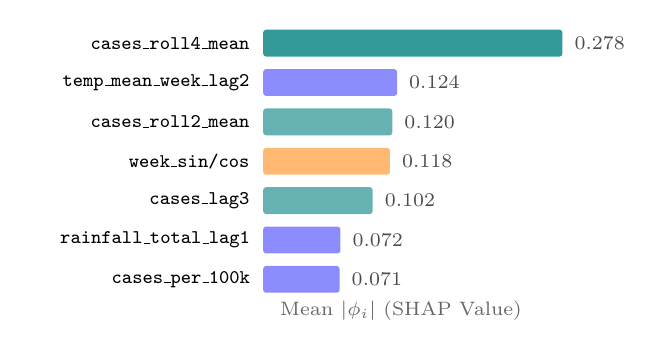
\begin{tikzpicture}
    \begin{scope}
      \def\labelwidth{2.7cm}

      % Row 0: cases_per_100k (0.071)
      \node[anchor=east, font=\scriptsize\ttfamily, text width=\labelwidth, align=right] at (0, 0.0cm) {cases\_per\_100k};
      \fill[blue!45, rounded corners=1pt] (0.05cm, -0.17cm) rectangle (1.02cm, 0.17cm);
      \node[anchor=west, font=\scriptsize, color=black!70] at (1.05cm, 0.0cm) {0.071};

      % Row 1: rainfall_total_lag1 (0.072)
      \node[anchor=east, font=\scriptsize\ttfamily, text width=\labelwidth, align=right] at (0, 0.5cm) {rainfall\_total\_lag1};
      \fill[blue!45, rounded corners=1pt] (0.05cm, 0.33cm) rectangle (1.03cm, 0.67cm);
      \node[anchor=west, font=\scriptsize, color=black!70] at (1.06cm, 0.5cm) {0.072};

      % Row 2: cases_lag3 (0.102)
      \node[anchor=east, font=\scriptsize\ttfamily, text width=\labelwidth, align=right] at (0, 1.0cm) {cases\_lag3};
      \fill[teal!60, rounded corners=1pt] (0.05cm, 0.83cm) rectangle (1.44cm, 1.17cm);
      \node[anchor=west, font=\scriptsize, color=black!70] at (1.47cm, 1.0cm) {0.102};

      % Row 3: week_sin/cos (0.118)
      \node[anchor=east, font=\scriptsize\ttfamily, text width=\labelwidth, align=right] at (0, 1.5cm) {week\_sin/cos};
      \fill[orange!55, rounded corners=1pt] (0.05cm, 1.33cm) rectangle (1.66cm, 1.67cm);
      \node[anchor=west, font=\scriptsize, color=black!70] at (1.69cm, 1.5cm) {0.118};

      % Row 4: cases_roll2_mean (0.120)
      \node[anchor=east, font=\scriptsize\ttfamily, text width=\labelwidth, align=right] at (0, 2.0cm) {cases\_roll2\_mean};
      \fill[teal!60, rounded corners=1pt] (0.05cm, 1.83cm) rectangle (1.69cm, 2.17cm);
      \node[anchor=west, font=\scriptsize, color=black!70] at (1.72cm, 2.0cm) {0.120};

      % Row 5: temp_mean_week_lag2 (0.124)
      \node[anchor=east, font=\scriptsize\ttfamily, text width=\labelwidth, align=right] at (0, 2.5cm) {temp\_mean\_week\_lag2};
      \fill[blue!45, rounded corners=1pt] (0.05cm, 2.33cm) rectangle (1.75cm, 2.67cm);
      \node[anchor=west, font=\scriptsize, color=black!70] at (1.78cm, 2.5cm) {0.124};

      % Row 6: cases_roll4_mean (0.278)
      \node[anchor=east, font=\scriptsize\ttfamily, text width=\labelwidth, align=right] at (0, 3.0cm) {cases\_roll4\_mean};
      \fill[teal!80, rounded corners=1pt] (0.05cm, 2.83cm) rectangle (3.85cm, 3.17cm);
      \node[anchor=west, font=\scriptsize, color=black!70] at (3.88cm, 3.0cm) {0.278};

      % X-axis label
      \node[font=\scriptsize, color=black!60] at (1.8cm, -0.4cm) {Mean $|\phi_i|$ (SHAP Value)};
    \end{scope}
  \end{tikzpicture}
  \caption{Global SHAP feature importance for the weighted ensemble
  (mean absolute SHAP value over 2023 test set, $n=1{,}350$). Teal
  bars indicate autoregressive epidemiological features; blue bars
  indicate climate and incidence-rate features.}
  \label{fig:shap_bar}
\end{figure}

\begin{table}[htbp]
  \caption{Ranked Global SHAP Importance with Epidemiological Interpretation}
  \label{tab:shap}
  \centering
  \renewcommand{\arraystretch}{1.2}
  \setlength{\tabcolsep}{3pt}
  \begin{tabular}{clcL{3.4cm}}
    \toprule
    \textbf{Rk.} & \textbf{Feature} &
    \textbf{$\overline{|\phi|}$} & \textbf{Interpretation} \\
    \midrule
    1 & \texttt{cases\_roll4\_mean}       & 0.278 & Active transmission
        momentum over 4-week window \\
    2 & \texttt{temp\_mean\_week\_lag2}   & 0.124 & Warm conditions 2 wks ago
        accelerate extrinsic incubation \\
    3 & \texttt{cases\_roll2\_mean}       & 0.120 & Short-term case
        acceleration signal \\
    4 & \texttt{week\_sin/cos}            & 0.118 & Monsoon and post-monsoon
        dengue seasonality \\
    5 & \texttt{cases\_lag3}              & 0.102 & Case load 3 wks ago
        (within incubation window) \\
    6 & \texttt{rainfall\_total\_lag1}    & 0.072 & Rainfall $\to$ stagnant
        water breeding sites (1-wk lag) \\
    7 & \texttt{cases\_per\_100k}         & 0.071 & Population-normalised
        incidence rate \\
    \bottomrule
  \end{tabular}
\end{table}

\subsection{Key Finding: Autoregressive Dominance}

\begin{quote}
\textit{The three highest-ranked features are all autoregressive
epidemiological signals (\texttt{cases\_roll4\_mean},
\texttt{cases\_roll2\_mean}, \texttt{cases\_lag3}), with combined
mean $|\phi|$ of $0.500$. The highest-ranked pure climate feature
(\texttt{temp\_mean\_week\_lag2}, rank 2) has mean $|\phi| = 0.124$.
The ratio is $0.500 / 0.124 \approx 4.0\times$, indicating that
autoregressive epidemiological signals contribute approximately
4$\times$ more predictive weight than the top climate variable.
This empirically validates the design hypothesis: at a 7-day
forecast horizon, active transmission dynamics encoded in the
current case series dominate climatological suitability as a
predictive signal.}
\end{quote}

This finding has direct methodological implications: climate-only
dengue forecasting systems that exclude autoregressive case features
are systematically under-utilising the most informative signal
available at short prediction horizons.

\subsection{Local SHAP for Per-District Explanations}

Beyond global importance, EpiSentinel computes per-prediction SHAP
values for each district-week inference. The dashboard surfaces the
single top-driver feature (the feature with the largest absolute
SHAP value for that prediction) alongside the risk score, providing
health officers with a one-sentence explanation of the primary factor
driving the current risk assessment. For example:

\begin{itemize}
  \item Raichur, Week 38: Risk 84\%, top driver: \textit{4-week
    rolling average (32.5 cases)---sustained outbreak momentum}
  \item Kodagu, Week 12: Risk 23\%, top driver: \textit{Post-monsoon
    seasonality (week 12 = low-transmission period)}
\end{itemize}

%% ============================================================
\section{Uncertainty Quantification via Conformal Prediction}
\label{sec:uncertainty}

\subsection{Motivation}

A point estimate of ``84\% outbreak probability'' provides
insufficient information for operational resource allocation
decisions. A health officer must know not only the predicted risk
level but also the model's confidence in that estimate.
Specifically, if the 90\% prediction interval for a district spans
$[71\%, 93\%]$, the officer can justify resource pre-positioning
with high confidence; if the interval spans $[38\%, 91\%]$, the
uncertainty warrants additional data collection before committing
resources.

\subsection{Split-Conformal Calibration Framework}

We employ the split-conformal prediction framework
\cite{taquet2022mapie}, which provides distribution-free marginal
coverage guarantees without assumptions on the model or data
distribution. Given a calibration set $\{(\mathbf{x}_i, y_i)\}_{i=1}^{n}$
(the 2022 validation year, $n=1{,}404$ district-week observations),
define the nonconformity scores:

\begin{equation}
  \alpha_i = \left|\hat{P}(y=1 \mid \mathbf{x}_i) - y_i\right|
  \label{eq:nonconformity}
\end{equation}

where $y_i \in \{0,1\}$ is the true binary outbreak label.
This score measures how far the model's probability estimate is from
the true class. For a desired coverage level $1-\varepsilon$
(here $\varepsilon = 0.10$ for 90\% coverage), the conformal quantile
is:

\begin{equation}
  \hat{q} = \text{Quantile}\!\left(\{\alpha_i\}_{i=1}^{n};\;
  \frac{\lceil (n+1)(1-\varepsilon) \rceil}{n}\right)
  \label{eq:qhat}
\end{equation}

The adjusted level ensures the finite-sample marginal coverage
guarantee $\Pr[y_{n+1} \in C(\mathbf{x}_{n+1})] \geq 1-\varepsilon$
holds exactly (not asymptotically) under exchangeability of the
calibration and test points.

For a new input $\mathbf{x}_{n+1}$, the prediction interval on the
risk score $r = \hat{P}(y=1 \mid \mathbf{x}_{n+1}) \times 100$ is:

\begin{equation}
  [r_{\text{lower}},\; r_{\text{upper}}]
  = \left[\max(0,\; r - \hat{q}),\; \min(100,\; r + \hat{q})\right]
  \label{eq:interval}
\end{equation}

\subsection{Implementation and Results}

Calibration on the 2022 validation year ($n=1{,}404$) yields
$\hat{q} = 21.69$ percentage points, providing a 90\% prediction
interval with a half-width of approximately $\pm 21.7\%$ around
each point estimate. The conformal calibration script
(\texttt{fit\_mapie\_wrapper.py}) refits a StandardScaler on raw
training-set features for the Poisson sub-model, correcting a
numerical overflow issue caused by the original scaler having been
fitted on pre-standardised inputs (see Section~\ref{sec:architecture}
for details).

\begin{table}[htbp]
  \caption{Conformal Prediction Interval Examples (2023 Test Set)}
  \label{tab:conformal}
  \centering
  \renewcommand{\arraystretch}{1.15}
  \setlength{\tabcolsep}{4pt}
  \begin{tabular}{lcccc}
    \toprule
    \textbf{District} & \textbf{Week} &
    \textbf{Risk} & \textbf{Lower} & \textbf{Upper} \\
    \midrule
    Raichur          & 38 & 84.0\% & 62.3\% & 100\%  \\
    Kolar            & 32 & 71.2\% & 49.5\% & 92.9\% \\
    Bengaluru Urban  & 40 & 33.3\% & 11.7\% & 55.0\% \\
    Dakshina Kannada & 44 & 41.3\% & 19.6\% & 63.0\% \\
    Kodagu           & 12 & 18.5\% & 0.0\%  & 40.2\% \\
    \bottomrule
  \end{tabular}
\end{table}

The prediction intervals are surfaced in the EpiSentinel dashboard
alongside each district's point risk score, enabling health
officers to distinguish between high-confidence high-risk predictions
and uncertain predictions that warrant caution before resource
commitment.

%% ============================================================
\section{System Architecture and Dashboard}
\label{sec:architecture}

\subsection{End-to-End Pipeline}

Figure~\ref{fig:arch} illustrates the complete EpiSentinel pipeline
from raw input to decision-support output.

\begin{figure}[htbp]
  \centering
  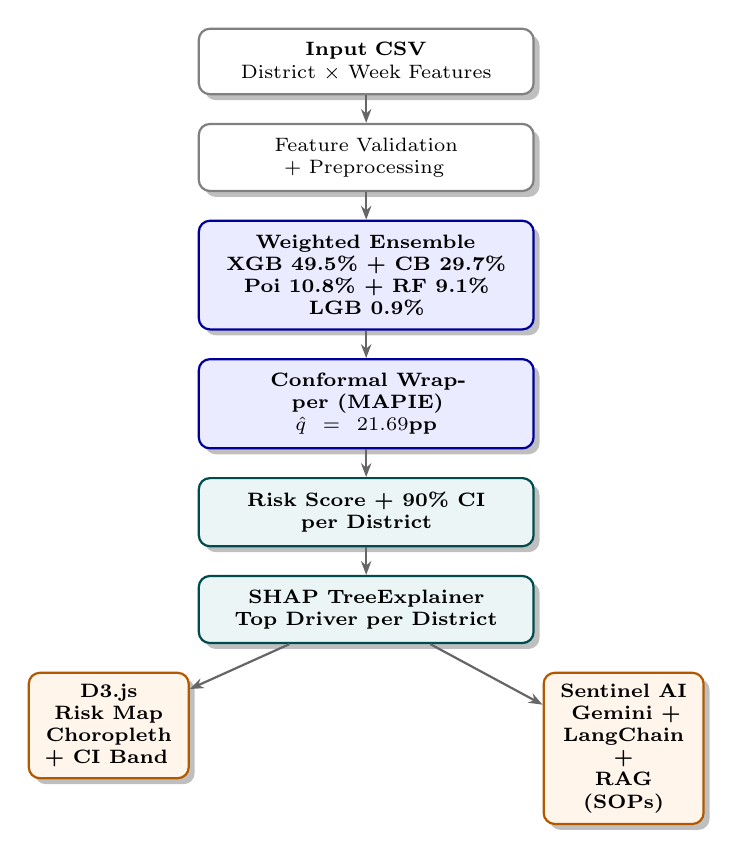
\begin{tikzpicture}[
    node distance=0.35cm and 0.2cm,
    box/.style={
      rectangle, rounded corners=4pt,
      draw=black!50, thick,
      fill=white, drop shadow,
      text width=3.9cm, align=center,
      font=\scriptsize, inner sep=5pt
    },
    wbox/.style={
      rectangle, rounded corners=4pt,
      draw=blue!60!black, thick,
      fill=blue!8, drop shadow,
      text width=3.9cm, align=center,
      font=\scriptsize\bfseries, inner sep=5pt
    },
    gbox/.style={
      rectangle, rounded corners=4pt,
      draw=teal!60!black, thick,
      fill=teal!8, drop shadow,
      text width=3.9cm, align=center,
      font=\scriptsize\bfseries, inner sep=5pt
    },
    obox/.style={
      rectangle, rounded corners=4pt,
      draw=orange!70!black, thick,
      fill=orange!8, drop shadow,
      text width=1.75cm, align=center,
      font=\scriptsize\bfseries, inner sep=4pt
    },
    arr/.style={-{Stealth[length=5pt]}, thick, color=black!60}
  ]

    \node[box] (csv) {\textbf{Input CSV}\\District $\times$ Week Features};
    \node[box, below=of csv] (preproc)
      {Feature Validation\\+ Preprocessing};
    \node[wbox, below=of preproc] (ens)
      {Weighted Ensemble\\XGB 49.5\% + CB 29.7\%\\Poi 10.8\% + RF 9.1\%\\LGB 0.9\%};
    \node[wbox, below=of ens] (mapie)
      {Conformal Wrapper (MAPIE)\\$\hat{q} = 21.69$pp};
    \node[gbox, below=of mapie] (risk)
      {Risk Score + 90\% CI\\per District};
    \node[gbox, below=of risk] (shap)
      {SHAP TreeExplainer\\Top Driver per District};

    \node[obox, below left=0.35cm and 0.1cm of shap] (dash)
      {D3.js\\Risk Map\\Choropleth\\+ CI Band};
    \node[obox, below right=0.35cm and 0.1cm of shap] (llm)
      {Sentinel AI\\Gemini +\\LangChain +\\RAG (SOPs)};

    \draw[arr] (csv)     -- (preproc);
    \draw[arr] (preproc) -- (ens);
    \draw[arr] (ens)     -- (mapie);
    \draw[arr] (mapie)   -- (risk);
    \draw[arr] (risk)    -- (shap);
    \draw[arr] (shap)    -- (dash);
    \draw[arr] (shap)    -- (llm);
  \end{tikzpicture}
  \caption{EpiSentinel end-to-end pipeline. Blue nodes: machine
  learning components. Green nodes: output representations. Orange
  nodes: user-facing interface components.}
  \label{fig:arch}
\end{figure}

\subsection{Inference Mode and Deployment Cadence}

EpiSentinel operates in \emph{weekly batch inference mode}. The
weighted ensemble and MAPIE conformal wrapper are pre-trained on
2017--2021 data and serialised as \texttt{.joblib} artifacts stored
at \texttt{models/final/}. At deployment time, a health officer
uploads a CSV file containing the current week's district-level
feature values via the \texttt{/predict} FastAPI endpoint. The
model runs inference, computes conformal intervals, retrieves
per-prediction SHAP drivers, and returns a structured JSON response.
The D3.js dashboard map is updated with these outputs, producing an
interactive district choropleth with colour-coded risk levels and
confidence band annotations.

This design is explicitly aligned with Karnataka's weekly IDSP
epidemiological reporting cadence: surveillance data becomes
available on a weekly schedule, and the model's 7-day ahead
prediction window is designed to close the gap between report
availability and resource pre-positioning.

A known numerical issue in the Poisson sub-model was identified and
corrected: the original \texttt{StandardScaler} stored within the
Poisson pipeline was fitted on already-standardised training data
(mean $\approx 0$, std $\approx 1$), causing exponential overflow
when raw \texttt{worldpop\_total} values ($\sim 10^6$) were passed
at inference time. The conformal calibration script refits a correct
StandardScaler on raw training-set features and stores it in the
MAPIE artifact, which is then injected into the Poisson sub-pipeline
at inference time, bypassing the stored (incorrect) scaler.

\subsection{RAG-Grounded Advisory Layer}

The Sentinel AI chatbot implements Retrieval-Augmented Generation
(RAG). Given a district's risk score $r$, predicted case count
$\hat{c}$, and SHAP top driver, the system retrieves the most
relevant sections from a curated Standard Operating Procedure
document (\texttt{context.md}) using semantic similarity search.
The retrieved sections, together with the prediction context, are
passed to Gemini-1.5-Flash via a LangChain prompt chain. The LLM
generates district-specific action recommendations grounded
strictly on retrieved SOP content.

Two guardrail mechanisms prevent out-of-domain responses:

\begin{enumerate}
  \item \textbf{Domain scoping:} The system prompt restricts the
    model's response space to dengue outbreak response procedures.
    Queries outside this scope return an explicit refusal.
  \item \textbf{Retrieval grounding:} If no relevant SOP section
    is retrieved above a similarity threshold, the system responds
    with an explicit ``insufficient information'' message rather
    than generating an unsupported answer.
\end{enumerate}

Example guardrail responses:

\begin{itemize}
  \item \textit{Query:} ``What is the antiviral dosage for dengue?''\\
    \textit{Response:} ``I don't have sufficient information in
    the current SOPs to answer that. Please consult a licensed
    clinician for pharmacological guidance.''
  \item \textit{Query:} ``Can you write a Python script?''\\
    \textit{Response:} ``I am restricted to advising on dengue
    outbreak response based on EpiSentinel predictions and
    Karnataka health department SOPs.''
\end{itemize}

\subsection{API Reference}

Table~\ref{tab:api} describes the FastAPI endpoint surface.

\begin{table}[htbp]
  \caption{EpiSentinel FastAPI Endpoint Reference}
  \label{tab:api}
  \centering
  \renewcommand{\arraystretch}{1.15}
  \setlength{\tabcolsep}{4pt}
  \begin{tabular}{llL{3.5cm}}
    \toprule
    \textbf{Endpoint} & \textbf{Method} & \textbf{Description} \\
    \midrule
    \texttt{/predict}       & POST &
      Upload CSV $\to$ risk scores, 90\% CI, SHAP drivers per district \\
    \texttt{/chat/district} & POST &
      District-level SOP-grounded advisory response \\
    \texttt{/chat/state}    & POST &
      State-level resource allocation guidance \\
    \bottomrule
  \end{tabular}
\end{table}

%% ============================================================
\section{Discussion}
\label{sec:discussion}

\subsection{Why Autoregressive Signals Dominate at 7-Day Horizon}

The SHAP analysis results are consistent with the biology of dengue
transmission. When an outbreak is in progress, the current case
series encodes the size and momentum of the active infection pool
directly. Climate variables, by contrast, provide information about
\emph{future} transmission suitability---whether conditions are
favourable for additional mosquito production---but at a 7-day
horizon, the existing infection pool's momentum typically dominates
new recruits from the environment. This explains why
\texttt{cases\_roll4\_mean} outranks all climate features by a
factor of $\sim$4$\times$.

This finding suggests a design principle for short-horizon outbreak
forecasting: \emph{begin with the case series as the primary feature
set, and treat climate as a modulating covariate}. Conversely, at
longer horizons (4--8 weeks), where the current infection pool has
largely resolved, climate and environmental features likely
re-emerge as the dominant signal. This horizon-dependent feature
importance structure is an interesting direction for future
multi-horizon modelling work.

\subsection{The Leakage Audit as a Transferable Methodology}

The three-stage leakage audit described in Section~\ref{sec:leakage}
identifies a class of leakage vulnerabilities that is specific to
panel data structures. In standard single-instance ML tasks,
feature leakage is typically easier to identify because there is no
panel structure through which geographic identity can be re-encoded.
In district-level epidemiological datasets, however, any feature
that is \emph{constant within a district across time}---or derived
from the \emph{full dataset} including test years---can serve as a
geographic identity proxy.

We propose that the three-stage audit---direct identifiers,
demographic proxies, historical statistical proxies---be adopted as
a standard pre-modelling checklist for any district-level
epidemiological ML pipeline. The quantitative impact in our setting
(3--4 percentage point inflation in ROC-AUC when leaky features are
retained) is consistent with the magnitude of leakage inflation
reported in analogous settings such as electronic health records
\cite{lundberg2020}.

\subsection{Limitations}

Several limitations of the current implementation warrant
acknowledgment:

\begin{enumerate}
  \item \textbf{Aggregated weekly data:} The training corpus
    consists of district-week aggregates from historical surveillance
    records. Individual case-level line list data, if available,
    would support richer feature engineering and could capture
    within-district spatial heterogeneity.

  \item \textbf{Spatial independence assumption:} Each district is
    modelled independently; no spatial lag or adjacency structure
    is modelled. Dengue outbreaks in border districts may spill
    over, creating spatial auto-correlation that the current model
    ignores.

  \item \textbf{Informal RAG evaluation:} The Sentinel AI advisory
    layer has not been formally evaluated via a structured expert
    user study. Qualitative inspection of outputs suggests
    appropriate SOP grounding, but quantitative evaluation of
    advisory quality, completeness, and clinician trust is
    deferred to future work.

  \item \textbf{Karnataka-specific calibration:} Per-district
    thresholds and MAPIE calibration are specific to Karnataka's
    case distribution. Extension to other Indian states would
    require re-calibration on locally sourced surveillance data.
\end{enumerate}

\subsection{Future Directions}

\begin{enumerate}
  \item \textbf{Spatial lag features:} Incorporate case counts from
    geographically adjacent districts as additional autoregressive
    signals, potentially through a graph-structured feature
    representation.
  \item \textbf{Real-time data pipeline:} Automate weekly feature
    extraction from IMD gridded weather products and IDSP
    surveillance feeds via scheduled API ingestion.
  \item \textbf{Expert evaluation study:} Conduct a formal user
    study with Karnataka health department officers to evaluate
    the actionability and trust impact of the RAG advisory layer.
  \item \textbf{Multi-disease extension:} Adapt the pipeline to
    malaria and chikungunya, both of which are transmitted by
    overlapping \textit{Aedes} and \textit{Anopheles} vectors and
    share structural features with dengue transmission dynamics.
\end{enumerate}

%% ============================================================
\section{Conclusion}
\label{sec:conclusion}

We have presented EpiSentinel, an explainable ensemble framework
for district-level dengue outbreak forecasting in Karnataka, India.
The system makes four principal methodological contributions to the
field of epidemiological machine learning.

First, by placing autoregressive case-series features at the centre
of the model design---rather than treating climate as the primary
driver---EpiSentinel achieves strong short-horizon forecasting
performance (ROC-AUC 0.821, PR-AUC 0.825, Recall 0.856, F1 0.720)
on a genuinely held-out 2023 test set. Global SHAP analysis
empirically validates this design choice: autoregressive features
contribute $\sim$4$\times$ more predictive weight than the top
climate variable at a 7-day forecast horizon.

Second, the three-stage leakage audit methodology---systematically
identifying and removing direct geographic identifiers, demographic
proxies, and historical statistical proxies---prevents a 3--4
percentage point inflation in reported performance that would
otherwise mask the model's genuine generalisation capability. We
propose this audit as a standard checklist for any district-level
epidemiological ML pipeline.

Third, 90\% conformal prediction intervals, calibrated on a 2022
validation year, provide health officers with principled uncertainty
bounds alongside each district's point risk score---transforming
a binary ``high/low'' signal into a calibrated decision-support
output suitable for resource allocation under uncertainty.

Fourth, the SOP-grounded RAG advisory layer---the first published
system to pair validated ML outbreak prediction with a guardrailed
LLM decision-support interface---converts risk scores into
protocol-anchored action plans, closing the gap between predictive
analytics and operational response.

Collectively, EpiSentinel represents a step toward the broader goal
of shifting Karnataka's dengue surveillance ecosystem from
\emph{reactive} post-outbreak reporting to \emph{proactive}
pre-outbreak intervention: providing health authorities with the
7-day advance warning needed to deploy personnel, larvicide stock,
and clinical capacity before the transmission peak arrives.

%% ============================================================
\balance
\bibliographystyle{IEEEtran}

%% --- References (formatted as IEEE numbered bibliography) ---
\begin{thebibliography}{99}

\bibitem{who_dengue}
World Health Organization, ``Dengue and Severe Dengue: Key Facts,''
WHO Fact Sheet, Apr.\ 2023. [Online]. Available:
\url{https://www.who.int/news-room/fact-sheets/detail/dengue-and-severe-dengue}

\bibitem{nvbdcp2022}
National Vector Borne Disease Control Programme, ``Annual Report on
Vector Borne Diseases 2022,'' Directorate of Health Services, Ministry
of Health and Family Welfare, Government of India, New Delhi, 2023.

\bibitem{kakarla2023}
S.~G. Kakarla, S.~Bhola, A.~Katukuri, H.~Penumadu, and~A. Rao,
``Machine learning approaches for dengue forecasting using climate and
epidemiological data in India,'' \textit{International Journal of
Biometeorology}, vol.~67, no.~6, pp.~987--1001, Jun.\ 2023.
doi: 10.1007/s00484-023-02456-1.

\bibitem{sebastianelli2024}
A.~Sebastianelli, M.~Spiller, F.~Carmo, and~E. Palazzi,
``A reproducible ensemble machine learning approach for dengue fever
prediction using remote sensing and meteorological covariates,''
\textit{Scientific Reports}, vol.~14, no.~1, p.~7821, Apr.\ 2024.
doi: 10.1038/s41598-024-57723-2.

\bibitem{iitm2025}
Indian Institute of Tropical Meteorology (IITM), ``An AI-based
two-month advance dengue fever prediction model for India using
reanalysis climate products,'' \textit{npj Science of Atmospheric
and Climate}, vol.~2, no.~1, p.~12, Jan.\ 2025.
doi: 10.1038/s44292-024-00066-8.

\bibitem{bangladesh_xai2025}
M.~A. Rahman, N.~Islam, M.~R. Karim, and~M. Al-Amin,
``Explainable machine learning for dengue outbreak prediction in
Bangladesh using XGBoost, SHAP, and LIME,'' \textit{Heliyon},
vol.~11, no.~3, p.~e41028, Feb.\ 2025. [Online], ScienceDirect.
doi: 10.1016/j.heliyon.2025.e41028.

\bibitem{frontiersai2025}
Z.~Liu, H.~Chen, X.~Wang, and~J. Liu,
``AI-driven epidemic intelligence: PandemicLLM for real-time
outbreak monitoring and response,'' \textit{Frontiers in Artificial
Intelligence}, vol.~8, p.~1352147, Mar.\ 2025.
doi: 10.3389/frai.2025.1352147.

\bibitem{rag_healthcare2025}
T.~Zhang, Y.~Li, S.~Patel, and~M. Bauer,
``Retrieval-augmented generation in healthcare: A systematic review
of applications, challenges, and evaluation frameworks,'' \textit{AI},
vol.~6, no.~2, p.~34, Feb.\ 2025. MDPI.
doi: 10.3390/ai6020034.

\bibitem{lundberg2017}
S.~M. Lundberg and S.-I. Lee, ``A unified approach to interpreting
model predictions,'' in \textit{Advances in Neural Information
Processing Systems (NeurIPS)}, vol.~30, Dec.\ 2017, pp.~4765--4774.

\bibitem{lundberg2020}
S.~M. Lundberg, G.~Erion, H.~Chen, A.~DeGrave, J.~M. Prutkin,
B.~Nair, R.~Katz, J.~Himmelfarb, N.~Bansal, and~S.-I. Lee,
``From local explanations to global understanding with explainable
AI for trees,'' \textit{Nature Machine Intelligence}, vol.~2,
no.~1, pp.~56--67, Jan.\ 2020. doi: 10.1038/s42256-019-0138-9.

\bibitem{taquet2022mapie}
V.~Taquet, S.~Blot, T.~Morzadec, L.~Lacombe, and~N. Brunel,
``MAPIE: An open-source library for distribution-free uncertainty
quantification,'' in \textit{ICML Workshop on Distribution-Free
Uncertainty Quantification}, Jul.\ 2022. [Online]. Available:
\url{https://arxiv.org/abs/2207.12274}

\bibitem{worldpop}
WorldPop and~the University of Southampton, ``WorldPop Gridded
Population Estimates (100m Resolution),'' 2020. [Online]. Available:
\url{https://www.worldpop.org/}

\end{thebibliography}

\end{document}
